\section{\'Etude d'un bénéfice (6 points)}

L'entreprise Ecolor est spécialisée dans la production et la vente de peinture éco-responsable. La production quotidienne varie entre 0 et 800 litres. Toute la production est vendue. Les montants de la recette et du coût sont exprimés en dizaines d'euros.

\begin{center}
	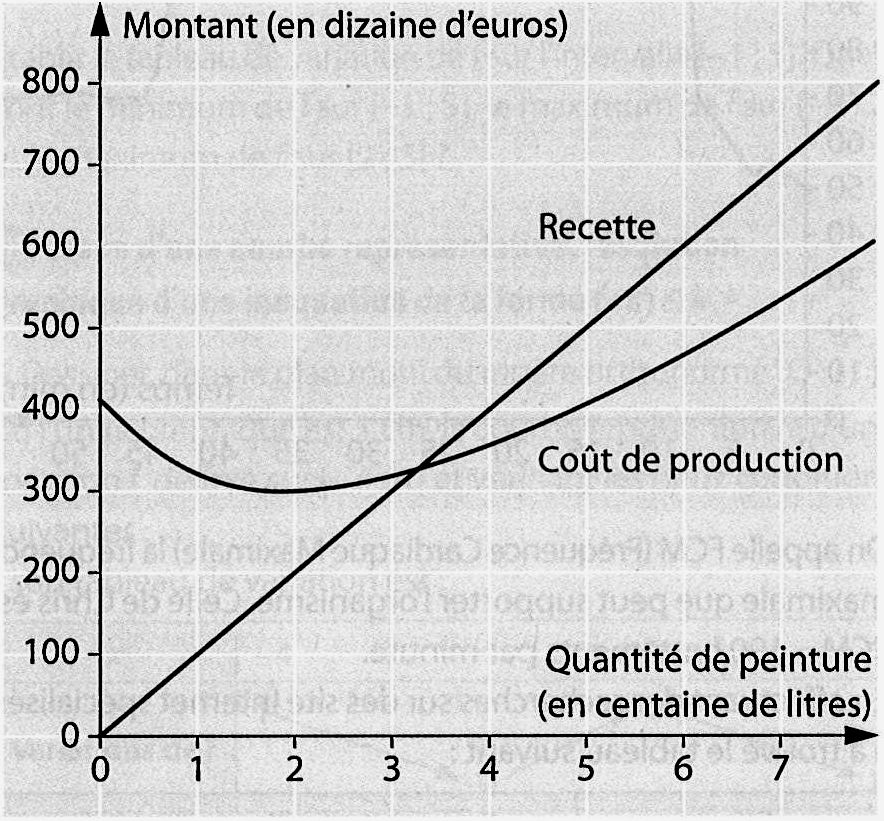
\includegraphics[scale=1.35]{img/graph}
\end{center}

A l'aide du graphique ci-dessus, répondre aux questions suivantes.
\begin{questions}
	\question[1] Déterminer le coût de production de 200 litres de peinture.
	\question[1] Quelle est la production de peinture pour avoir une recette de \num{5000} € ?
	
	\question[2] Déterminer l'équation de la droite correspondant aux recettes de l'entreprise.
	
	\question[1] A partir de combien de litres de peinture vendus, l'entreprise fait-elle un bénéfice ?
	
	\question[1] L'entreprise peut-elle réaliser un bénéfice de plus de 3000 € pour une production quotidienne variant entre 0 et 800 litres ?
\end{questions}